% !TEX root = ../main.tex

\section{Star Network Model}
\label{sec:star-network}

\scaffold{
  \textbf{Paragraph 1, the model.} Every pedal of \cref{sec:pedal-wiring} is a passive network between three terminals. Any such network is externally equivalent to three resistors meeting in one inner node, the star point \cite{kennelly1899equivalence}, as drawn in \cref{fig:star-network}. Define the term \emph{arm}: the resistance between one contact and the star point, written $r_\mathrm{T}$, $r_\mathrm{R}$ and $r_\mathrm{S}$ for tip, ring and sleeve. Use \enquote{arm} throughout, never \enquote{branch} or \enquote{leg}. State that the internal topology cannot be recovered from the terminals, only this equivalent \cite{borcea2012resistor}; the star form is chosen over the triangle form because, with one terminal open, a pair resistance is simply the sum of two arms.
}

\begin{figure}[htbp]
  \centering
  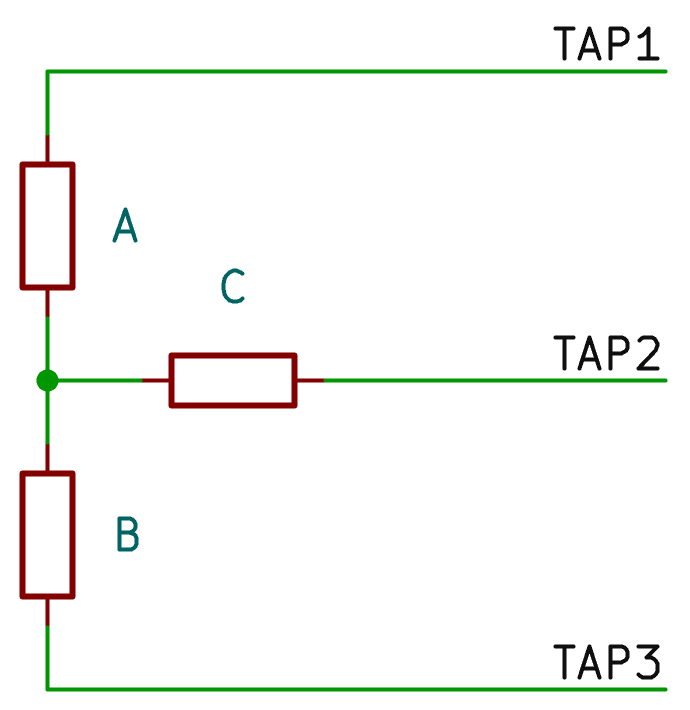
\includegraphics[width=0.3\linewidth]{03-measurement-principle/figures/star-network}
  \titledcaption{Star Network Model}{\scaffoldinline{Say that A, B and C are the three arms meeting in the star point and TAP1 to TAP3 the accessible contacts. Consider redrawing with the labels of the text ($r_\mathrm{T}$, $r_\mathrm{R}$, $r_\mathrm{S}$; tip, ring, sleeve), so that figure and text use one notation.}}
  \label{fig:star-network}
\end{figure}

\scaffold{
  \textbf{Paragraph 2, what the arms mean.} Translate the pedal types into arm values: a potentiometer is the case with exactly one arm near \qty{0}{\ohm}, the wiper, while the other two arms hold the two track sections; the ratio of these two is the position. A wiper resting on a track end additionally shorts that end to the star point (end stop). A two-wire pedal has an isolated arm. Conclude: identifying a pedal reduces to solving for three arm resistances and asking which are near zero or isolated.
}

\scaffold{
  \textbf{Paragraph 3, representation.} The solver reports the arms as relative values $q_i = r_i / R_\mathrm{tot}$ (summing to one) plus the total $R_\mathrm{tot} = \sum_i r_i$, because the ratios are measured far more precisely than the total (\cref{sec:pair-measurement}). Special values use the IEEE~754 encoding: $0$ for an arm shorted to the star point, $\infty$ for an isolated arm, NaN for an arm that is finite but cannot be separated from its partner, which happens when only two contacts are connected. Mention that this keeps the arithmetic closed, so no special cases propagate through the code.
}
